\documentclass{controle}
\usepackage{main}

% \printanswers{}

\title{Controle n°4 : Probabilités, vecteurs}
\author{Seconde 3}
\date{20 Février 2026}

\begin{document}
\titleandname{}
\instructions{}
\begin{questions}
\titledquestion{Probabilités}[5]
Dans une entreprise, les postes sont répartis d'après le tableau suivant :
\begin{center}
\begin{tblr}{hlines, vlines, columns={1.5cm,c}, rows={0.75cm,m}, column{1}={2.5cm,c}, row{1}={1cm,t}}
\diagbox[width=2.5cm,height=1cm]{Poste}{Genre}&Homme&Femme&Total\\
Technicien&350&250&600\\
Cadre&100&300&400\\
Total&450&550&1000
\end{tblr}
\end{center}
On interroge une personne au hasard à propos de son salaire. On suppose que le tirage est équiprobable. On définit les événements suivants.
\begin{itemize}
\item $F$ : \og La personne interrogée est une femme \fg 
\item $C$ : \og La personne interrogée est cadre \fg 
\end{itemize}
\begin{parts}
\part[1] Calculer $P(F)$ et $P(C)$.
\part[1] Calculer $P(F \cap C)$.
\part[1] En déduire $P(F \cup C)$.
\part[1] Calculer $P(\overbar{F \cup C})$ et $P(\overbar{F} \cap \overbar{C})$. Que remarquez-vous ?
\part[1] Une enquête plus précise interroge spécifiquement les femmes. Dans ce cas, quelle est la probabilité d'interroger une technicienne ?
\end{parts}

\begin{solution}[0.5cm]
\begin{parts}
\part $P(F) = \dfrac{550}{1000} = 0.55$ et $P(C) = \dfrac{400}{1000} = 0.4$
\part $F \cap C$ : \og La personne interrogée est une femme ET une cadre\fg.

Donc $P(F \cap C) = \dfrac{300}{1000} = 0.3$.
\part $F \cup C$ : \og La personne interrogée est une femme OU est cadre\fg

On utilise la formule du cours $P(F \cup C) = P(F) + P(C) - P(F \cap C) = 0.55 + 0.4 - 0.3 = 0.65$. 

On pourra sinon compter les cases correspondantes $P(F \cup C) = \dfrac{250 + 300 + 100}{1000} = 0.65$.
\part On peut utiliser la formule du cours $P(\overline{F \cup C}) = 1 - P(F \cup C) = 1 - 0.65 = 0.35$.

$\overline{F} \cap \overline{C}$ : \og La personne interrogée n'est ni une femme ni cadre \fg. Donc, on s'intéresse ici aux hommes techniciens.

Ainsi, $P(\overline{F} \cap \overline{C}) = \dfrac{350}{1000} = 0.35$.

Les deux probabilités sont égales.

\part Ici, on ne considère que les femmes avant de procéder à l'expérience. Ainsi, la probabilité d'interroger une technicienne parmi les femmes est de $\dfrac{250}{550} = \dfrac{25}{55}$.
\end{parts}
\end{solution}

\titledquestion{Vecteurs et translations}[5]
Sur la figure suivante, les quadrilatères $ABCD$, $BEFC$, $DCHG$ et $CFIH$ sont des parrallélogrammes semblables (de même dimensions).
\begin{center}
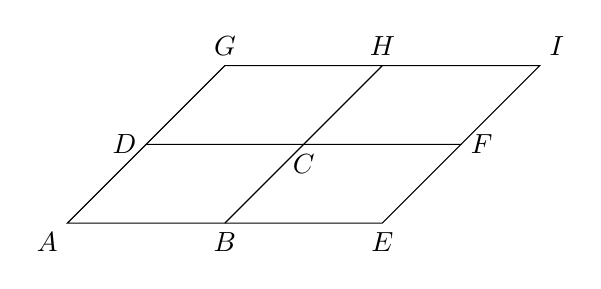
\begin{tikzpicture}
\coordinate (A) at (0,0);
\coordinate (B) at (2,0);
\coordinate (C) at (3,1);
\coordinate (D) at (1,1);
\coordinate (E) at (4,0);
\coordinate (F) at (5,1);
\coordinate (G) at (2,2);
\coordinate (H) at (4,2);
\coordinate (I) at (6,2);

\draw (A) -- (B) -- (C) -- (D) -- cycle;
\draw (B) -- (E) -- (F) -- (C);
\draw (D) -- (G) -- (H) -- (C);
\draw (H) -- (I) -- (F);
\draw (A) node[below left] {$A$};
\draw (B) node[below] {$B$};
\draw (C) node[below] {$C$};
\draw (D) node[left] {$D$};
\draw (E) node[below] {$E$};
\draw (F) node[right] {$F$};
\draw (G) node[above] {$G$};
\draw (H) node[above] {$H$};
\draw (I) node[above right] {$I$};
\end{tikzpicture}
\end{center}

Dans cet exercice, on ne demande aucune justification. Nommer un vecteur égal au vecteurs suivants :
\begin{parts}
\begin{minipage}{0.45\textwidth}
\part[0,5] $\vect{AD} =$  
\part[0,5] $\vect{FC} =$
\part[0,5] $\vect{CI} =$
\part[0,5] $- \vect{BC} =$
\part[0,5] $2 \vect{BA} =$
\end{minipage}
\hfill
\begin{minipage}{0.45\textwidth}
\part[0,5] $\vect{GH} + \vect{HC} =$
\part[0,5] $\vect{FC} + \vect{CB} =$
\part[0,5] $\vect{DA} - \vect{EA} =$
\part[0,5] $\vect{BH} + \vect{GC} + \vect{DB} =$
\part[0,5] $\vect{DB} - \vect{HF} =$
\end{minipage}
\end{parts}

\begin{solution}[0.5cm]
Les solutions proposées sont des exemples, ce ne sont pas les seuls réponses valables.
\begin{parts}
\begin{minipage}{0.45\textwidth}
\part[0,5] $\vect{AD} = \vect{BC}$  
\part[0,5] $\vect{FC} = \vect{IH}$
\part[0,5] $\vect{CI} = \vect{BF}$
\part[0,5] $- \vect{BC} = \vect{DA}$
\part[0,5] $2 \vect{BA} = \vect{IG}$
\end{minipage}
\hfill
\begin{minipage}{0.45\textwidth}
\part[0,5] $\vect{GH} + \vect{HC} = \vect{GC}$
\part[0,5] $\vect{FC} + \vect{CB} = \vect{FB}$
\part[0,5] $\vect{DA} - \vect{EA} = \vect{DE}$
\part[0,5] $\vect{BH} + \vect{GC} + \vect{DB} = \vect{AE}$
\part[0,5] $\vect{DB} - \vect{HF} = \vect{0}$
\end{minipage}
\end{parts}
\end{solution}
\titledquestion{Vecteurs et algèbre}[5]
\begin{parts}
\part[0,5] Rappeler la relation de Chasles en recopiant et complétant l'égalité suivante :
\begin{equation*}
\vect{A\dots} + \vect{B\dots} = \vect{AC}
\end{equation*}
\part[0,5] Soit $\vect{u}$ et $\vect{v}$ deux vecteurs tels qu'il existe un nombre $k$ tel que $\vect{u} = k \times \vect{v}$. Que peut-on dire de la direction de $\vect{u}$ et $\vect{v}$ ?
\part À partir des égalités suivantes, trouver $k$ tel que $\vect{AB} = k\vect{AC}$.
\begin{subparts}
\subpart[0,5] $\vect{AB} = \vect{CA}$
\subpart[0,5] $\vect{AB} = 7\vect{AC} + 3\vect{CA}$
\subpart[1] $\vect{AB} + \vect{AC} = 2\vect{AB} - 5\vect{AC}$
\subpart [1] $\vect{AB} + \vect{AC} = 3\vect{BC}$ (Indication : on utilisera $\vect{BC} = \vect{BA} + \vect{AC}$)
\subpart [1] $3\vect{CB} = 2\vect{AB}$ (Indication : on utilisera $\vect{CB} = \vect{CA} + \vect{AB}$)
\end{subparts}
\end{parts}
\begin{solution}
\begin{parts}
\part $\vect{AB} + \vect{BC} = \vect{AC}$.
\part Les vecteurs $\vect{u}$ et $\vect{v}$ ont la même direction : on dit qu'ils sont colinéaires.
\part
\begin{subparts}
\subpart $\vect{AB} = \vect{CA} = - \vect{AC}$, donc $k = -1$.
\subpart $\vect{AB} = 7\vect{AC}+ 3\vect{CA} = 7\vect{AC} - 3\vect{AC} = 4\vect{AC}$, donc $k = 4$.
\subpart
\begin{equation*}
\begin{aligned}
&\vect{AB} + \vect{AC} = 2\vect{AB} - 5\vect{AC}\\
\Leftrightarrow& \vect{AB} - 2\vect{AB} = -5\vect{AC} - \vect{AC}\text{ (On regroupe les termes)}\\
\Leftrightarrow& -\vect{AB} = -6\vect{AC} \text{ (On réduit)}\\
\Leftrightarrow& \vect{AB} = 6\vect{AC}\text{ (On divise par $-1$ des deux côtés)}\\
\end{aligned}
\end{equation*}
Donc $k = 6$
\subpart
\begin{equation*}
\begin{aligned}
&\vect{AB} + \vect{AC} = 3\vect{BC}\\
\Leftrightarrow&\vect{AB} + \vect{AC} = 3(\vect{BA} + \vect{AC}) \text{ (On utilise l'indication)}\\
\Leftrightarrow&\vect{AB} + \vect{AC} = 3\vect{BA} + 3\vect{AC} \text{ (On développe)}\\
\Leftrightarrow&\vect{AB} - 3\vect{BA} = 3\vect{AC} - \vect{AC}\text{ (On regroupe les termes)}\\
\Leftrightarrow&\vect{AB} + 3\vect{AB} = 3\vect{AC} - \vect{AC}\text{ (Car $\vect{BA} = - \vect{AB}$)}\\
\Leftrightarrow&4\vect{AB} = 2\vect{AC}\text{ (On réduit)}\\
\Leftrightarrow&\vect{AB}=\dfrac{1}{2}\vect{AC}\text{ (On divise par $4$)}
\end{aligned}
\end{equation*}
Donc $k = \dfrac{1}{2}$
\subpart
\begin{equation*}
\begin{aligned}
&3\vect{CB}=2\vect{AB}\\
\Leftrightarrow&3(\vect{CA} + \vect{AB})=2\vect{AB}\text{ (On utilise l'indication)}\\
\Leftrightarrow&3\vect{CA} + 3\vect{AB}=2\vect{AB}\text{ (On développe)}\\
\Leftrightarrow&3\vect{CA}=2\vect{AB} - 3\vect{AB}\text{ (On regroupe les termes)}\\
\Leftrightarrow&-3\vect{AC}=2\vect{AB} - 3\vect{AB}\text{ (On utilise $\vect{CA} = -\vect{AC}$)}\\
\Leftrightarrow&-3\vect{AC}=-\vect{AB}\text{ (On réduit)}\\
\Leftrightarrow&3\vect{AC}=\vect{AB}\text{ (On divise par $-1$)}\\
\end{aligned}
\end{equation*}
Donc $k = 3$.
\end{subparts}
\end{parts}
\end{solution}
\titledquestion{Vecteurs et Modélisation}[5]
Soit $ABC$ un triangle quelconque. Soient $D$ et $E$ deux points tels que $\vect{AD} = \dfrac{1}{4}\vect{AB}$ et $\vect{AE}=4\vect{AC}$
\begin{parts}
\part[1] Construire le triangle $ABC$ ainsi que le points $D$ et $E$.
\part[1] En utilisant l'égalité $\vect{DC} = \vect{DA} + \vect{AC}$, montrer que
\begin{equation*}
\vect{DC} = \vect{AC} - \dfrac{1}{4}\vect{AB}
\end{equation*}
\part[1] En utilisant l'égalité $\vect{BE} = \vect{BA} + \vect{AE}$, montrer que
\begin{equation*}
\vect{BE} = 4\vect{AC} - \vect{AB}
\end{equation*}
\part[1] Déduire des questions précédentes que $\vect{BE} = 4\vect{DC}$.
\part[1] En déduire la nature du quadrilatère $BECD$.
\end{parts}
\begin{solution}
\begin{parts}
\part
\part On part de l'égalité $\vect{DC} = \vect{DA} + \vect{AC}$. Alors,
\begin{equation*}
\begin{aligned}
\vect{DC} &= \vect{DA} + \vect{AC}\\ 
&= -\vect{AD} + \vect{AC}\\
&= -(\dfrac{1}{4}\vect{AB}) + \vect{AC}\\
&= \vect{AC} - \dfrac{1}{4}\vect{AB}
\end{aligned}
\end{equation*}
\part On part de l'égalité $\vect{BE} = \vect{BA} + \vect{AE}$. Alors,
\begin{equation*}
\begin{aligned}
\vect{BE} &= \vect{BA} + \vect{AE}\\ 
&= \vect{BA} + (4\vect{AC})\\
&= -\vect{AB} + (4\vect{AC})\\
&= 4\vect{AC} - \vect{AB}
\end{aligned}
\end{equation*}
\part On part de $4\vect{DC}$ pour montrer l'égalité de l'énoncé.
\begin{equation*}
\begin{aligned}
4\vect{DC} &= 4(\vect{AC} -\dfrac{1}{4}\vect{AB})\\
&= 4\vect{AC} - 4 \times \dfrac{1}{4} \vect{AB}\\
&= 4\vect{AC} - \vect{AB}\\
&= \vect{BE}
\end{aligned}
\end{equation*}
Ainsi, $\vect{BE} = 4\vect{DC}$.
\part Le quadrilatère $BECD$ est un trapèze.
\end{parts}

\end{solution}
\end{questions}
\end{document}